\documentclass[12pt,a4paper]{report}
\usepackage[affil-it]{authblk}
\usepackage{amsthm}
\usepackage{amssymb}
\usepackage{amsmath}
\usepackage{listings}
\usepackage{graphicx}
\usepackage{pgfplots}
\usepackage{float}
\usepackage{xcolor}
\usepackage{hyperref}
\usepackage{algpseudocode}
\usepackage[nameinlink]{cleveref}

\usepackage[
  backend=biber,
  style=alphabetic,
  sorting=anyt,
  minnames=3,
  minalphanames=3
]{biblatex}

\hypersetup{
    colorlinks=true,
    citecolor=blue,
    linkcolor=blue,
    urlcolor=blue,
    pdftitle={Computational Complexity Homework 2024-25},
}
\RequirePackage{enumitem}

\newtheorem{question}{Question}
\theoremstyle{definition}
\newtheorem{solution}{Solution}

\definecolor{sapRed}{HTML}{6f0a19}
\definecolor{sapBlue}{HTML}{006778}
\usetikzlibrary{automata,arrows}

\newcommand{\curlyquotes}[1]{\textquotedblleft #1\textquotedblright}
\newcommand{\abs}[1]{\left|#1\right|}
\newcommand{\abk}[1]{\left\langle#1\right\rangle}
\newcommand{\ceil}[1]{\left\lceil#1\right\rceil}

\newcommand{\N}{\mathbb{N}}
\newcommand{\func}[3]{#1 : #2 \to #3}
\newcommand{\funcmap}[5]{#1 : #2 \to #3 : #4 \mapsto #5}

\addbibresource{./references.bib}

\begin{document}

    \setlength{\parskip}{5pt}               % Vertical spacing between paragraphs
    \setlength{\parindent}{0pt}             % Vertical spacing between paragraphs

    \title{Computational Complexity \\ Homework 2024-25}
    \author{Simone Bianco, 1986936}
    \affil{Sapienza Università di Roma, Italy}
    \date{\today}

    \maketitle

    \textbf{Esercizio 1.1}

    \begin{center}
        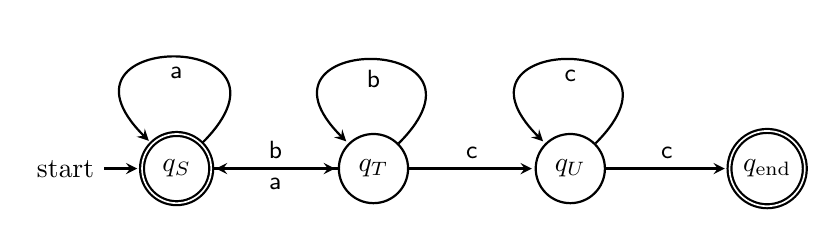
\begin{tikzpicture}[->,>=stealth,shorten >=1pt,auto,node distance=2.5cm,thick,main node/.style={scale=0.9,circle,draw,font=\sffamily\normalsize}]
            \node[initial,state,accepting] (0) {$q_S$};
            \node[state] (1) [right of=0] {$q_T$};
            \node[state] (2) [right of=1] {$q_U$};
            \node[state, accepting] (3) [right of=2] {$q_{\mathrm{end}}$};
 
            \path[every node/.style={font=\sffamily\small}]
                (0) edge [loop] node { a} (0)
                (0) edge [] node { b} (1)
                (1) edge [loop] node { b} (1)
                (1) edge  node { a} (0)
                (1) edge [] node { c} (2)
                (2) edge [loop] node { c} (2)
                (2) edge [] node { c} (3)
             ;
         \end{tikzpicture}
    \end{center}

    \textbf{Esercizio 1.2}
    
    \textit{Enunciato:} Se $L$ è un linguaggio regolare allora esiste un $p \in \N$ tale che $\forall w \in L$ con $\abs{w} \geq p$ esistono tre stringhe $x,y,z \in \Sigma^*$ per cui $w = xyz$ e:
    \begin{enumerate}
        \item $\forall i \in \N$ vale che $xy^iz \in L$
        \item $\abs{y} > 0$
        \item $\abs{xy} \leq p$
    \end{enumerate}

    \textit{Dimostrazione:} 

        Dato $L \in \mathsf{REG}$, sia $D := (Q, \Sigma, \delta, q_0, F)$ il DFA tale che $L=L(D)$
        
        Sia $p:= \abs{Q}$. Data la stringa $w := w_1 \ldots w_n \in L$ dove $w_1, \ldots, w_n \in \Sigma$ e dove $n \geq p$, consideriamo la sequenza di stati $r_1,\ldots, r_{n+1}$ tramite cui $w$ viene accettata da $D$:
        \[\forall k \in [1,n] \;\; \delta(r_k,w_k) = r_{k+1}\]
        Notiamo quindi che $\abs{r_1, \ldots, r_{n+1}} = n+1$, ossia che il numero di stati attraversati sia $n+1$. Inoltre, in quanto $n \geq p$, ne segue automaticamente che $n+1 \geq p+1$. Tuttavia, poiché $p := \abs{Q}$ e $n+1 \geq p+1$, ne segue necessariamente che $\exists i, j \mid 1 \leq i < j \leq p+1 \land r_i = r_j$, ossia che tra i primi $p+1$ stati della sequenza vi sia almeno uno stato ripetuto
        
        A questo punto, consideriamo le seguenti sottostringhe di $w$:
        \begin{itemize}
            \item $x = w_1 \ldots w_{i-1}$, tramite cui si ha che $\delta^*(r_1, x) = r_i$
            \item $y = w_i \ldots w_{j-1}$, tramite cui si ha che $\delta^*(r_i, y) = r_j = r_i$
            \item $z = w_j \ldots w_{n}$, tramite cui si ha che $\delta^*(r_j, z) = r_{n+1}$
        \end{itemize}
        
        Poiché $\delta^*(r_i, y) = r_i$, ossia $y$ porta sempre $r_i$ in se stesso, ne segue automaticamente che
        \[\forall k \in \N \;\; \delta^*(r_i, y^k) = r_i \implies \delta(r_1, xy^kz) = r_{n+1} \in F \implies xy^kz \in L(D) = L\]
        
        Inoltre, ne segue direttamente che $\abs{y} > 0$ in quanto $i < j$ e che $\abs{xy} \leq p$ in quanto $j \leq p+1$


        \textit{Esempio di applicazione:}


        Consideriamo il linguaggio $L = \{0^n1^n \mid n \in \N\}$. Supponiamo per assurdo che $L$ sia regolare. In tal caso, ne segue che per esso debba valere il pumping lemma, dove $p$ è la lunghezza del pumping. Consideriamo quindi la stringa $w := 0^p1^p \in L$. Poiché $\abs{w} \geq p$, possiamo suddividerla in tre sottostringhe $x,y,z \in \Sigma^*$ tali che $w = xyz$, 

        Poiché la terza condizione del pumping lemma impone che $\abs{xy} \leq p$ e poiché $w := 0^p1^p$, ne segue che $xy = 0^m$ e $z = 0^{p-m}1^{p}$, dove $m \in [1,p]$
        Inoltre, per la seconda condizione del lemma, si ha che $\abs{y} > 0$, dunque necessariamente si ha che $x = 0^{m-k}$ e $y = 0^k$, dove $k \in [1,m]$
        
        A questo punto, consideriamo la stringa $xy^0z$. Notiamo immediatamente che
        \[xy^0z = 0^{m-k} (0^k)^0 0^{p-m}1^{p} = 0^{m-k} 0^{p-m}1^{p} = 0^{p-k} 1^p\]
        implicando dunque che $xy^0z \notin L$, contraddicendo la prima condizione del lemma per cui si ha che $\forall i \in \N \;\; xy^iz \in L$. Dunque, ne segue necessariamente che $L$ non possa essere regolare.


        \newpage

        \textbf{Esercizio 2.1}

        \textit{Dimostrazione}:

        Sia $\func{f}{\Sigma^*}{\Sigma^*}$ la funzione calcolata dalla \textsf{TM} $F$ definita come segue.
            
        $F$ = "Data la stringa $\abk{M,w}$ in input:
        \begin{enumerate}[label={\arabic*. }]
            \item Costruisci una \textsf{TM} $M'$ definita come:
            
            $M'$ = "Data la stringa $x$ in input:
            \begin{enumerate}[label={\roman*. }]
                \item Esegui il programma di $M$ su input $w$.
                \item Se $M$ accetta, $M'$ \textit{accetta}. Se $M$ rifiuta, $M'$ va in loop.
            \end{enumerate}
            \item Restituisci in output la stringa $\abk{M'}$"
        \end{enumerate}

        Supponiamo che $\abk{M,w} \in A_\textsf{TM}$. In tal caso, per ogni input $x$ la macchina $M'$ accetterà sempre, implicando che essa sia un decisore e dunque che $\abk{M'} \in \mathrm{DECIDER}_{TM}$.

        Viceversa, supponiamo che $\abk{M,w} \not A_\textsf{TM}$. In tal caso, abbiamo due opzioni: $M(w)$ rifiuterà oppure andrà in loop. Se $M(w)$ rifiuta allora $M'(x)$ andrà in loop. Se invece $M(w)$ va in loop, allora anche $M'(x)$ andrà in loop poiché esegue $M(w)$ al suo interno. In entrambi i casi la macchina risulta non essere un decisore, dunque $\abk{M'} \notin \mathrm{DECIDER}_{TM}$. Ciò conclude che $f$ sia una riduzione da $A_{TM}$ a $\mathrm{DECIDER}_{TM}$. Inoltre, poiché $A_{TM}$ è indecidibile, concludiamo che anche $\mathrm{DECIDER}_{TM}$ deve necessariamente essere indecidibile.

        \textbf{Esercizio 2.2}

        \textit{Dimostrazione:}

        Sia $\prec$ una relazione che ordina le stringhe di $\Sigma^*$ in base alla loro lunghezza e (a parità di lunghezza) in base al loro ordine lessico-grafico.
        
        Sia quindi $\func{f}{\N}{\Sigma^*}$ la funzione definita come:
        \[f(i) = \text{$i$-esima stringa di $\Sigma^*$ secondo $\prec$}\]
        
        Poiché $\prec$ è un ordine totale, tale funzione risulta essere biettiva, implicando che $\abs{\N} = \abs{\Sigma^*}$. Consideriamo quindi il linguaggio $\mathcal{M} \subseteq \Sigma^*$ definito come:
        \[\mathcal{M} = \{\abk{M} \mid M \text{ è una \textsf{TM}}\}\]
        Poiché $\mathcal{M} \subseteq \Sigma^*$ e $\Sigma^*$ è numerabile, ne segue automaticamente che anche $\abs{\N} = \abs{\mathcal{M}}$. Consideriamo quindi l'insieme $\mathcal{L} = \mathcal{P}(\Sigma^*)$, corrispondente all'insieme di tutti i linguaggi definiti su $\Sigma$. Dato $L \in \mathcal{L}$, definiamo la sequenza binaria $\chi_L = b_1b_2\ldots$ come:
        \[b_i = \begin{array}{ll}
            1 & \text{ se } s_i \in L\\
            0 & \text{ se } s_i \notin L\\
        \end{array}\]

        dove $s_1, s_2, \ldots$ sono tutte le stringhe di $\Sigma^*$ ordinate secondo $\prec$. Consideriamo quindi la seguente funzione:
        \[\funcmap{g}{\mathcal{L}}{\mathcal{B}}{L}{\chi_Ldefinita}\]

        Anche tale funzione è biettiva, implicando che $\abs{\mathcal{L}} = \abs{\mathcal{B}}$. Di conseguenza, poiché $\mathcal{B}$ non è numerabile, ne segue che anche $\mathcal{L}$ non sia numerabile. A questo punto, poiché $\mathcal{M}$ è numerabile e $\mathcal{L}$ no, concludiamo che la seguente funzione:
        \[\funcmap{h}{\mathcal{M}}{\mathcal{L}}{M}{L(M)}\]
        non possa essere biettiva, implicando che $\exists L \in \mathcal{L} \mid \nexists M \in \mathcal{M} \text{ t.c } L = L(M)$


        \newpage

        \textbf{Esercizio 3.1}

        \textit{Dimostrazione:}

        Procederemo in modo simile al padding argument che dimostra come se $\mathsf{P} = \mathsf{NP}$ allora $\mathsf{EXP} = \mathsf{NEXP}$. Dato un linguaggio $L \in \mathrm{NTIME}(n^5)$, sia $V$ il verificatore per $L$ con runtime $O(n^5)$. Consideriamo il linguaggio $L_{pad} = \{x\#1^{{\abs{x}}^{\frac{5}{2}}} \mid x \in L\}$ e definiamo il seguente verificatore $V_{pad}$:
        
        $V_{pad}$ = "Dati $x$ e $w$ in input:
        \begin{enumerate}
            \item Controlla se $x = y\#1^{{\abs{y}}^{\frac{5}{2}}}$ per qualche stringa $y$.
            \item Se falso, rifiuta.
            \item Se vero, esegui $V(y,w)$ e ritorna il suo risultato"
        \end{enumerate}

        Poiché l'input di $V_{pad}$ ha dimensione $m = \abs{y\#1^{{\abs{y}}^{\frac{5}{2}}}}$, la prima istruzione di $V_{pad}$ richiede tempo $O(m)$, mentre l'ultima istruzione può essere eseguita in tempo $O(m^2)$. Ciò conclude che $L_{pad} \in \mathrm{NTIME}(n^2)$.
        
        Di conseguenza, sotto l'assunzione $\mathrm{DTIME}(n^2) = \mathrm{NTIME}(n^2)$, ne segue che esiste un decisore $M_{pad}$ per $L_{pad}$ con runtime $O(n^2)$. Costruiamo quindi una nuova TM definita come:

        $M$ = "Dato $x$ in input:
        \begin{enumerate}
            \item Costruisci la stringa $y = x\#1^{{\abs{x}}^{\frac{5}{2}}}$.
            \item Esegui $M_{pad}(y)$ e ritorna il suo risultato.
        \end{enumerate}

        Chiaramente $M$ risulta essere un decisore per $L$. Inoltre, per via della costruzione della stringa $y$, il suo runtime risulta essere $O(n^5)$, concludendo che $L \in \mathrm{DTIME}(n^5)$.


        \newpage

        \textbf{Esercizio 3.2}

        \textit{Dimostrazione:}

        Per definizione delle due classi sappiamo già che $\mathrm{PSPACE} \subseteq \mathrm{NPSPACE}$. Per ottenere l'altra inclusione, dimostriamo il teorema di Savitch, il quale afferma che $\mathrm{NSPACE}(f(n)) \subseteq \mathrm{DSPACE}(f^2(n))$.

        Sia $N$ una \textsf{NTM} tale che $L(N) \in \mathrm{NSPACE}(f(n))$. Assumiamo $N$ abbia un solo stato accettante $q_\mathrm{accept}$. Sia inoltre $q_\mathrm{start}$ lo stato iniziale di $N$. Dato un input $w$, consideriamo quindi il grafo delle configurazioni $G_{N,w}$ per $N(w)$ definito come:
        \begin{itemize}
            \item Ad ogni nodo di $V$ corrisponde una configurazione possibile di $N$ durante la computazione di $w$
            \item Per ogni nodo $v_i, v_j \in V$, esiste un arco se e solo se la computazione può passare dalla configurazione $c_i$ alla configurazione $c_j$ tramite $\delta$
        \end{itemize}
        
        Definiamo quindi la seguente procedura $\mathtt{PathG_{N,w}?}(x,y,k)$:

        $\mathtt{PathG_{N,w}?}(x,y,k)$:

        \begin{enumerate}[label={\arabic*.}]
            \item Se $k = 0$, verifica se $(x,y) \in E(G_{N,w})$ o se $x=y$. Se vero, \textit{accetta}. Altrimenti, \textit{rifiuta}
            \item Se $k > 0$, ripeti la seguente istruzione per ogni nodo $v$ in $V(G_{N,w})$:
            \begin{enumerate}[label={\arabic*.}, start=3]
                \item Se $\mathtt{PathG_{N,w}?}(x,v,k-1)$ accetta e $\mathtt{PathG_{N,w}?}(v,y,k-1)$ accetta, allora la procedura \textit{accetta}. Altrimenti, essa \textit{rifiuta}
            \end{enumerate}
        \end{enumerate}

        Per costruzione stessa di $\mathtt{Path?}$, si ha che:
        \[\mathtt{Path?}(x,y,k) \text{ accetta} \iff \text{Esiste cammino $x \to y$ di massimo $2^k$ nodi}\]

        Il costo in termini di spazio per questa procedura risulta essere $O(\log^2 k)$, dove $k$ è il valore dato in input alla prima chiamata della procedura. Definiamo quindi la seguente TM $M$:
        
        $M$ = "Data la stringa $w$ in input:
        \begin{enumerate}
            \item Esegui la procedura $PathG_{N,w}?(c_\mathrm{start}, c_\mathrm{accept}, \ceil{\log m})$ costruendo il grafo $G_{N,w}$ durante la sua esecuzione (conservando sempre solo il nodo attuale e successivo)
            \item Se la procedura accetta, \textit{accetta}. Altrimenti, \textit{rifiuta}"
        \end{enumerate}

        Per costruzione stessa di $M$, si ha che:
        \[w \in L(M) \iff PathG_{N,w}?(c_\mathrm{start}, c_\mathrm{accept}, \ceil{\log 2^{f(n)}}) \text{ accetta} \iff\]
        \[\text{Esiste cammino } c_\mathrm{start} \to c_\mathrm{accept} \text{ di $2^{f(n)}$ nodi in } G_{N,w} \iff w \in L\]
        implicando che $L(M) = L$. Notiamo quindi che la costruzione parziale del grafo richieda solo qualche "variabile" di appoggio, mantenendo il costo della procedura inalterato in termini di spazio, ossia pari a $O(\log^2 2^{f(n)}) = O(f^2(n))$, concludendo che $L \in \mathrm{DSPACE}(f^2(n))$


\end{document}